\documentclass[11pt,a4paper]{article}

\usepackage[utf8]{inputenc}
\usepackage[T1]{fontenc}
\usepackage{lmodern}
\usepackage[provide=*,spanish]{babel}
\usepackage[a4paper,margin=2.35cm,headheight=15pt]{geometry}
\usepackage{microtype}
\usepackage{booktabs}
\usepackage{tabularx}
\usepackage{longtable}
\usepackage{array}
\usepackage{xcolor}
\usepackage{hyperref}
\usepackage{xurl}
\usepackage{enumitem}
\usepackage{listings}
\usepackage{fancyhdr}
\usepackage{parskip}
\usepackage{needspace}
\usepackage{graphicx}
\usepackage{pdfpages}
\usepackage{pgf-umlsd}

\definecolor{ucaldasink}{HTML}{2D3142}
\definecolor{ucaldasslate}{HTML}{4F5D75}
\definecolor{ucaldasaccent}{HTML}{BF4520}
\definecolor{ucaldasrule}{HTML}{D8DADF}

\hypersetup{
  colorlinks=true,
  linkcolor=ucaldasink,
  urlcolor=ucaldasaccent,
  citecolor=ucaldasink,
  pdftitle={Gestión de Monitores Académicos},
  pdfauthor={Equipo del proyecto}
}

\setlength{\parindent}{0pt}
\setlength{\parskip}{0.55em}
\setlist[itemize]{leftmargin=1.5em,itemsep=0.2em,topsep=0.25em}
\setlist[enumerate]{leftmargin=1.7em,itemsep=0.25em,topsep=0.25em}
\renewcommand{\arraystretch}{1.2}
\newcolumntype{Y}{>{\raggedright\arraybackslash}X}

\lstdefinestyle{comandos}{
  basicstyle=\ttfamily\small,
  breaklines=true,
  breakatwhitespace=false,
  columns=fullflexible,
  keepspaces=true,
  showstringspaces=false,
  frame=single,
  rulecolor=\color{ucaldasrule},
  backgroundcolor=\color{black!3},
  xleftmargin=0.4em,
  xrightmargin=0.4em,
  aboveskip=0.6em,
  belowskip=0.6em,
  literate=
    {á}{{\'a}}1 {é}{{\'e}}1 {í}{{\'i}}1 {ó}{{\'o}}1 {ú}{{\'u}}1
    {Á}{{\'A}}1 {É}{{\'E}}1 {Í}{{\'I}}1 {Ó}{{\'O}}1 {Ú}{{\'U}}1
    {ñ}{{\~n}}1 {Ñ}{{\~N}}1 {ü}{{\"u}}1 {Ü}{{\"U}}1
}
\lstset{style=comandos}

\pagestyle{fancy}
\fancyhf{}
\fancyhead[L]{\small Gestión de Monitores Académicos}
\fancyhead[R]{\small Universidad de Caldas}
\fancyfoot[L]{\small Ingeniería de Software III · 2026-2}
\fancyfoot[R]{\small Página \thepage}
\renewcommand{\headrulewidth}{0.4pt}
\renewcommand{\footrulewidth}{0.4pt}

\newcommand{\portada}[2]{%
  \hypersetup{pageanchor=false}
  \begin{titlepage}
    \centering
    \vspace*{2.5cm}
    {\large Universidad de Caldas\par}
    \vspace{0.5cm}
    {\large Ingeniería de Software III · 2026-2\par}
    \vspace{2.5cm}
    {\Huge\bfseries Gestión de Monitores Académicos\par}
    \vspace{0.7cm}
    {\LARGE #1\par}
    \vspace{0.7cm}
    {\large #2\par}
    \vfill
    {\large Versión 1.0 · 20 de noviembre de 2026\par}
    \vspace{0.4cm}
    {\normalsize Equipo del proyecto\par}
  \end{titlepage}
  \hypersetup{pageanchor=true}
  \pagenumbering{roman}
}

\newcommand{\codigo}[1]{\texttt{#1}}
\newcommand{\archivo}[1]{\path{#1}}
\newcommand{\componente}[1]{\texttt{#1}}


\begin{document}

\portada{Documento final}{Gestión de Monitores Académicos}

\tableofcontents
\clearpage
\pagenumbering{arabic}

\section{Introducción}

Este documento reúne, en un solo archivo, la documentación del proyecto Gestión de Monitores Académicos: arquitectura, diagramas, manual técnico, manual de usuario y el contrato de API. Está listo para entregar y subir.

\section{Diagrama de arquitectura}

\begin{figure}[htbp]
\centering
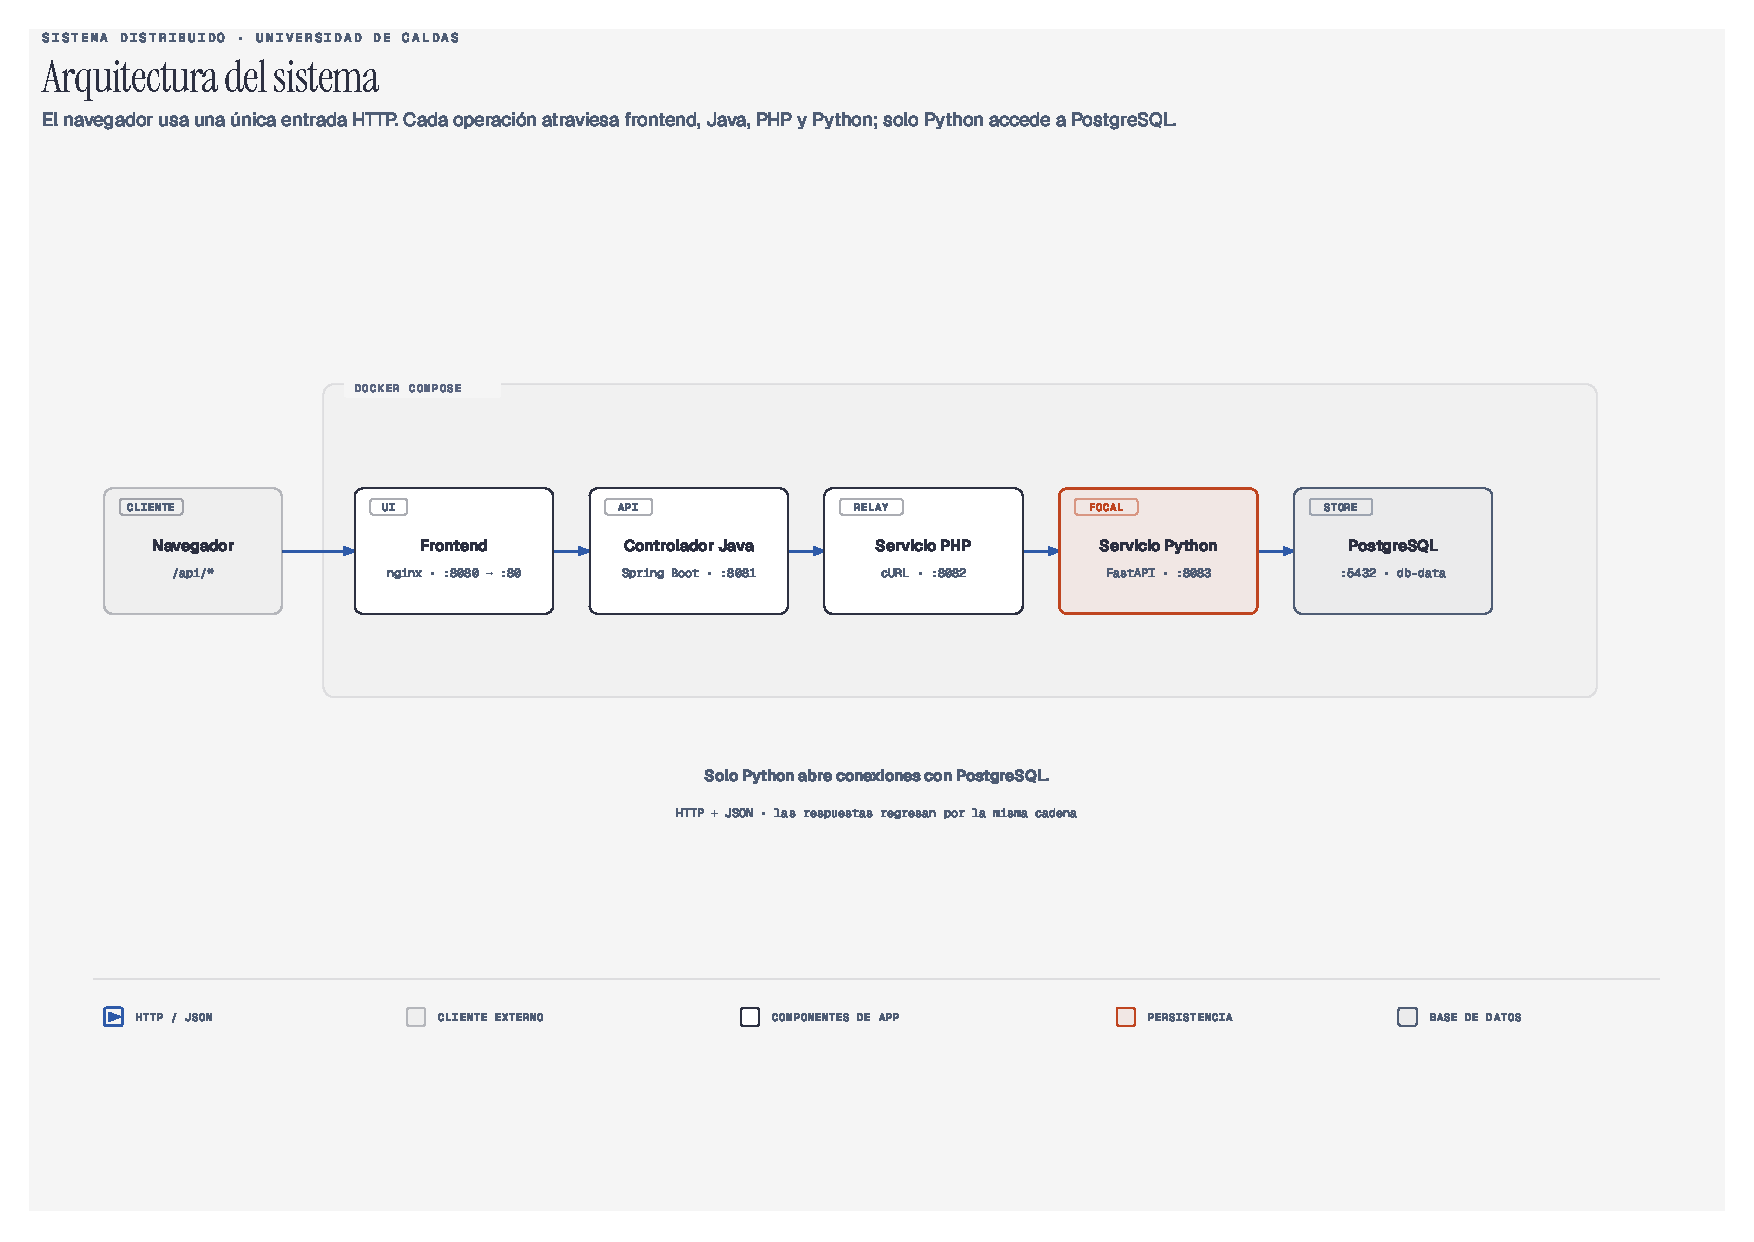
\includegraphics[width=\textwidth,height=0.70\textheight,keepaspectratio]{arquitectura.pdf}
\caption{Arquitectura distribuida, multicapa y heterogénea. El navegador usa una única entrada HTTP y solo Python accede a PostgreSQL.}
\label{fig:arquitectura}
\end{figure}

\section{Patrones y estilos arquitectónicos}

\begin{tabularx}{\textwidth}{p{0.20\textwidth}p{0.39\textwidth}Y}
\toprule
\textbf{Patrón / estilo} & \textbf{Cómo funciona} & \textbf{Componentes y justificación} \\
\midrule
Capas (layered) & Cada capa tiene una responsabilidad y se comunica con la siguiente mediante HTTP y JSON. El recorrido del CRUD no salta componentes. & \textbf{Componentes:} frontend, Java, PHP, Python y PostgreSQL. \textbf{Por qué:} separa presentación, validación, intermediación y persistencia, y deja trazable cada operación. \\
Cliente-servidor & Un cliente inicia una petición y un servidor la atiende; el cliente no conoce la implementación interna del servidor. & \textbf{Componentes:} el navegador es el cliente; nginx, Java, PHP y Python responden como servidores HTTP/JSON. \textbf{Por qué:} la interfaz consume una API estable sin acoplarse a los procesos internos. \\
Microservicios (aplicación backend) & Los servicios backend se despliegan y se ejecutan de manera independiente y se comunican por red, sin compartir memoria. & \textbf{Componentes:} Java, PHP y Python son servicios independientes; PostgreSQL es el almacén de datos que los respalda, no un microservicio. \textbf{Por qué:} cada tecnología ejecuta una responsabilidad acotada y puede evolucionar manteniendo el contrato común. \\
REST & Los recursos se identifican por URI, usan métodos HTTP estandarizados y representan datos en JSON sin mantener estado entre peticiones. & \textbf{Componentes:} los endpoints de \componente{materias} y \componente{monitores}. \textbf{Por qué:} el contrato define una interfaz uniforme para el CRUD y la comunicación entre capas. \\
Proxy inverso y mismo origen & nginx recibe el tráfico del navegador, elimina el prefijo \codigo{/api} y reenvía la petición a Java. El navegador nunca accede a los servicios internos. & \textbf{Componentes:} nginx en el frontend. \textbf{Por qué:} centraliza la entrada HTTP, evita CORS y no expone los hosts internos ni la base de datos. \\
Repository / DAO & La persistencia se encapsula en un módulo que recibe una conexión y ejecuta SQL parametrizado; quien lo invoca decide el alcance de la transacción. & \textbf{Componentes:} \componente{repository.py} en Python. \textbf{Por qué:} concentra el acceso a PostgreSQL, separa reglas de negocio de SQL y evita concatenar valores en las consultas. \\
\bottomrule
\end{tabularx}

\section{Ventajas y dificultades de la arquitectura distribuida y heterogénea}

\subsection{Ventajas}
\begin{itemize}
  \item \textbf{Responsabilidades separadas:} cada componente tiene un límite claro y puede evolucionar sin reescribir las demás capas, siempre que respete el contrato común.
  \item \textbf{Pruebas focalizadas:} una falla de validación, intermediación o persistencia puede aislarse en la capa correspondiente y verificarse sin atribuir el error a toda la aplicación.
  \item \textbf{Expresividad tecnológica:} Java, PHP, Python y PostgreSQL se utilizan según la responsabilidad asignada, mostrando una arquitectura heterogénea en lugar de repetir la misma tecnología en todas las capas.
  \item \textbf{Punto de entrada controlado:} nginx mantiene al navegador en el mismo origen y evita exponer los puertos internos o el acceso directo a la base de datos.
  \item \textbf{Contrato verificable:} el smoke test recorre el flujo completo y comprueba códigos y mensajes, por lo que una incompatibilidad entre capas se detecta de extremo a extremo.
\end{itemize}

\subsection{Dificultades}
\begin{itemize}
  \item \textbf{Latencia y disponibilidad:} cada operación cruza varios procesos y red; la indisponibilidad de cualquier eslabón impide completar la petición.
  \item \textbf{Riesgo de deriva contractual:} Java, PHP y Python deben conservar rutas, cuerpos y códigos HTTP; una diferencia entre capas produce respuestas inconsistentes.
  \item \textbf{Complejidad operativa:} se deben desplegar cinco contenedores, configurar red, volúmenes, variables y tiempos de espera, y respetar el orden de arranque saludable.
  \item \textbf{Diagnóstico distribuido:} un error puede originarse en cualquier salto, por lo que se necesitan logs por servicio, trazas correlacionadas y pruebas de la cadena completa.
  \item \textbf{Acceso único a datos:} solo Python puede escribir en PostgreSQL; cualquier intento de acceso directo desde otra capa rompe el control de transacciones y validación.
\end{itemize}

\section{Diagrama de secuencia: registro de un monitor}

\begin{figure}[htbp]
\centering
\resizebox{\textwidth}{!}{%
\begin{sequencediagram}
\newinst{navegador}{Navegador}
\newinst{nginx}{nginx / frontend}
\newinst{java}{Controlador Java}
\newinst{php}{Servicio PHP}
\newinst{python}{Servicio Python}
\newinst{db}{PostgreSQL}

\mess{navegador}{POST /api/monitores [datos]}{nginx}
\mess{nginx}{POST /monitores [datos]}{java}
\begin{call}{java}{normalizar y validar campos}{java}{datos válidos o error 400}
\end{call}

\begin{sdblock}[lightgray]{Camino exitoso: HTTP 201}{La respuesta regresa por la misma cadena}
\begin{call}{java}{reenviar POST /monitores}{php}{201}
  \begin{call}{php}{reenviar POST /monitores}{python}{201}
    \begin{call}{python}{consultar materia}{db}{existe}
    \end{call}
    \begin{call}{python}{insertar monitor}{db}{creada}
    \end{call}
  \end{call}
\end{call}
\mess{java}{201 monitor creado a nginx}{nginx}
\mess{nginx}{201 monitor creado al navegador}{navegador}
\end{sdblock}

\begin{sdblock}[lightgray]{Alternativa 400: datos inválidos}{Java responde sin llamar a PHP}
\mess{java}{400 JSON inválido o campo obligatorio}{nginx}
\mess{nginx}{400 error de validación al navegador}{navegador}
\end{sdblock}

\begin{sdblock}[lightgray]{Alternativa 409: código duplicado}{Python traduce el error de PostgreSQL}
\mess{db}{UniqueViolation de PostgreSQL}{python}
\mess{python}{409 código duplicado a PHP}{php}
\mess{php}{409 código duplicado a Java}{java}
\mess{java}{409 código duplicado a nginx}{nginx}
\mess{nginx}{409 código duplicado al navegador}{navegador}
\end{sdblock}
\end{sequencediagram}%
}
\caption{Alternativas del registro de un monitor: creación 201, validación 400 en Java y conflicto 409 generado en PostgreSQL y propagado por Python, PHP y Java.}
\label{fig:secuencia-registro}
\end{figure}

\section{Endpoints de la API}

\begin{tabularx}{\textwidth}{p{0.14\textwidth}p{0.40\textwidth}p{0.16\textwidth}Y}
\toprule
\textbf{Método} & \textbf{Ruta en la API pública} & \textbf{Éxito} & \textbf{Uso} \\
\midrule
\codigo{GET} & \codigo{/api/health} & 200 & Estado de Java a través del frontend. \\
\codigo{GET} & \codigo{/api/materias} & 200 & Lista materias de solo lectura. \\
\codigo{GET} & \codigo{/api/monitores} & 200 & Lista monitores; sin resultados devuelve \codigo{[]}. \\
\codigo{GET} & \codigo{/api/monitores/\{codigo\}} & 200 & Consulta un monitor por código. \\
\codigo{POST} & \codigo{/api/monitores} & 201 & Crea un monitor. \\
\codigo{PUT} & \codigo{/api/monitores/\{codigo\}} & 200 & Reemplaza los campos editables; no cambia el código. \\
\codigo{DELETE} & \codigo{/api/monitores/\{codigo\}} & 204 & Elimina el monitor sin cuerpo de respuesta. \\
\bottomrule
\end{tabularx}

Los errores tienen formato \codigo{\{"error": "mensaje"\}}. Estados principales: \codigo{400} para datos inválidos o materia inexistente, \codigo{404} para monitor o ruta inexistente, \codigo{405} para método no permitido, \codigo{409} para código duplicado, \codigo{502} ante indisponibilidad de un servicio descendente, \codigo{503} ante indisponibilidad de PostgreSQL y \codigo{500} para errores no previstos. El catálogo completo de mensajes y el orden de validación están en \archivo{docs/api-contract.md}.

\section{Documentos incluidos}

A continuación se incluyen los documentos completos del proyecto:


\includepdf[pages=-]{manual-tecnico.pdf}


\includepdf[pages=-]{manual-usuario.pdf}

\section{Documentos relacionados}

\begin{itemize}
  \item \archivo{docs/api-contract.md}: contrato normativo de API, rutas, JSON, validaciones, mensajes de error y esquema de base de datos.
  \item \archivo{CONTRIBUTING.md}: reglas de trabajo del equipo (ramas, commits, PRs, versiones y estilo).
  \item \archivo{README.md}: instrucciones de ejecución y solución de problemas.
\end{itemize}

\end{document}
